% EDIT HISTORY:
%2017 a1 version: added references recommended in referee report from JCTA; del conjecture.
%2017 a2 version: changed address of first author


%2018 a3: some changes due to SIAM referee
%2018 a4: more changes.


    \synctex=1	

\documentclass[a4paper,12pt]{article}
\usepackage[vcentermath]{youngtab}
%\usepackage[dvips]{graphicx}
\usepackage{amsmath, epsfig, cite}
\usepackage{amssymb}
\usepackage{amsfonts}
\usepackage{latexsym}
%\usepackage{graphicx}
\usepackage{extarrows}
\usepackage{booktabs}
\usepackage{color}

\usepackage[inline]{showlabels}   %%% this command shows label beside equations in PDF

\usepackage{tikz}
\usetikzlibrary{calc,through,backgrounds}
%
%\makeatletter\textsc{\textsc{}}
%\newcommand{\rmnum}[1]{\romannumeral #1}
%\newcommand{\Rmnum}[1]{\expandafter\@slowromancap\romannumeral #1@}
%\makeatother


\def\proof{\noindent {\it{Proof.} \hskip 2pt}}
\def \remark {\noindent \emph{Remark. }}

\newtheorem{thm}{Theorem}[section]
\newtheorem{prop}[thm]{Proposition}
\newtheorem{property}[thm]{Property}
\newtheorem{cor}[thm]{Corollary}
\newtheorem{defi}[thm]{Definition}
 %\newtheorem{def}[thm]{Definition}
\newtheorem{lem}[thm]{Lemma}
\newtheorem{conj}[thm]{Conjecture}
\newtheorem{problem}[thm]{Problem}
\newtheorem{openproblem}[thm]{Open Problem}
\newtheorem{question}[thm]{Question}
\newtheorem{exam}[thm]{\it Example}
\renewcommand{\thefootnote}{\fnsymbol{footnote}}
\renewcommand{\thefigure}{\arabic{section}.\arabic{figure}}
\newcommand{\qed}{{\hfill\rule{4pt}{7pt}}}
\def\pf{\noindent {\it Proof.} }
\def\R{{\widetilde{R}}}




\makeatletter \@addtoreset{equation}{section} \makeatother

\setlength{\textwidth}{155mm} \setlength{\textheight}{23cm}
\setlength{\headheight}{3cm} \setlength{\topmargin}{0pt}
\setlength{\headsep}{0pt} \setlength{\oddsidemargin}{0pt}
\setlength{\evensidemargin}{0pt}

\parindent 15pt
\voffset -25mm \rm
\parskip=6pt


%%%%
%%%%%%%%%%%%%%%%%%%%%%%%%%%%%%%%%%
%%%%%  Here is preamble for TPX, which is all sort of bullshit and crap.
%%%%%%%%%%%%%%%%%%%%%%%%%%%%%%%%%%
%%%%
\usepackage{color}
%\pdfoutput=0 % uncomment this if running PDFTeX in TeX mode
\usepackage{ifpdf}
%\ifx\pdftexversion\undefined %if using TeX
%  \usepackage{graphicx}
%\else %if using PDFTeX
%  \usepackage[pdftex]{graphicx}
%\fi
\ifpdf %if using PDFTeX in PDF mode
  \DeclareGraphicsExtensions{.pdf,.png,.mps}
  \usepackage{pgf}
\else %if using TeX or PDFTeX in TeX mode
  \usepackage{graphicx}
  \DeclareGraphicsExtensions{.eps,.bmp}
  \DeclareGraphicsRule{.emf}{bmp}{}{}% declare EMF filename extension
  \DeclareGraphicsRule{.png}{bmp}{}{}% declare PNG filename extension
  \usepackage{pgf}
  \usepackage{pstricks}%variant: \usepackage{pst-all}
\fi
\usepackage{epic,bez123}
\usepackage{floatflt}% package for floatingfigure environment
\usepackage{wrapfig}% package for wrapfigure environment


\begin{document}
\rule{0cm}{1cm}
\begin{center}
{\Large\bf The Corners of Core Partitions }
\end{center}
 \vskip 6mm
 \begin{center}
{\small
Harry H.Y. Huang$^1$ and Larry X.W. Wang$^2$}
\vskip 4mm $^{1}$Center for Applied Mathematics,\\
Tianjin University, Tianjin 300072, P.R. China \\[3mm]
\vskip 4mm $^{2}$Center for Combinatorics, LPMC-TJKLC\\
Nankai University, Tianjin 300071, P.R. China \\[3mm]
\vskip 4mm
%$^1$chen@nankai.edu.cn,
$^1$haoyang.huang@tju.edu.cn,
$^2$wsw82@nankai.edu.cn \end{center}


\begin{abstract}




In this paper, we are concerned with the corners of core partitions. We introduce the concepts of stitches and anti-stitches, certain pairs of cells in a quotient space which we call wrap-up space. We prove that the anti-stitches of a rational Dyck path are in bijection with the segments of structure sets of the corresponding core partition, therefore the number of corners of a core partition can be counted by the number of stitches or anti-stitches. %We also give a rational version of Cycle Lemma .
Based on these results, for coprime positive integers $a$ and $b$, we give two essentially different formulae for the number of corners in all $(a,b)$-cores. This leads to an unexpected identity, expressing the rational Catalan numbers as weighed sums of binomial numbers.
Moreover, we show that for an $(n,n+1)$-core partition $\lambda$  determined by a certain $(n,n+1)$-Dyck path $P$, the corners of $\lambda$ correspond to pairs of consecutive right steps in $P$.
As a consequence, we show that the number of $(n,n+1)$-cores with $k$ corners is the  Narayana number $N(n,k+1)$. We also extend these results to multi-cores.
\end{abstract}



\noindent {\bf Keywords}: core partitions, Dyck paths, Cycle Lemma, corners of a partition, Narayana number

\noindent {\bf AMS Subject Classification}: 05A17, 05A19

\section{Introduction}

%The study of integer partitions has been an active field of research in the past decades. Integer partitions play an important role in combinatorics and have deep connections with other branches of mathematics such as representation theory and number theory.


The objective of this paper is to investigate the  number of corners  of core partitions.
Recall that a partition of a positive integer $n$ is a finite non-increasing sequence of positive integers of sum $n$.
The number of distinct parts of a partition, i.e., the number of corners in its Ferrers diagram, has attracted many researchers.
Goh and Schmutz \cite{GS95} gave a central limit theorem for the number of different parts in a random integer partition. Lovejoy \cite{lovejoy01} studied the arithmetic properties of partitions with distinct parts. Ono \cite{Ono98} gave  weighted recurrence relations  for the number of partitions of $n$ with distinct parts.

%
%              Can't find much in the literature about corners!
%
%%_______ \emph{(give more example about the number of corners, not the partition with distinct parts; especially george andrews)}

%And
%One simple yet beautiful property of this value is that the number of corners of partitions of $n$ are equally distributed with the number of $1$s in partitions of $n$.
%
%More generally, we have the following theorem:
%
%\begin{thm}
%The number of $k$'s and number of parts that appear at least $k$ times in a partition  are equally distributed over partitions of $n$.
%\end{thm}
%
%Richard Stanley first noticed it and included it as an exercise in his distinguished book \textbf{EC1} \cite{EC1}.
%______this theorem is really important? Do we need this theorem in the remaining? if not, I think we can delete it_____

The corner statistic has been also touched upon in the well-developed theory of overpartitions. Corteel and  Lovejoy \cite{lovejoy04} introduced the overpartitions, which are partitions where each corner has a label chosen from two possible labels.
Lovejoy \cite{lovejoy04b} related  overpartitions to Andrews' combinatorial generalization of the Gollnitz-Gordon identities and a theorem of Andrews and Santos on partitions with attached odd parts.
Lovejoy and Bringmann \cite{lovejoy09} studied overpartition analogues of Ramanujan's mock theta function. They showed that these functions are related to the generating function of certain Hurwitz class numbers.
%to the generating function for Hurwitz class numbers $H(n)$ of binary quadratic forms of discriminant $-n$.


%%%%%%%%%%%%%%%%%%%%%%% ÖÎѧҪÑϽ÷£¬ÕâЩÎÄÏ×Ҫϸ¶Á¡£

In this paper, we will be concerned with the corners of core partitions. Recall that a partition is a $t$-core partition (or a $t$-core for short) if none of its cells has hook length divisible by $t$.  The notion of $t$-core arise from the study of modular representations. Nakayama  \cite{nakayama} first conjectured that two characters of $S_n$ are in the same $p$-block if and only if they are labelled by partitions with the $p$-core (the $p$-core of a given partition is obtained by repeatedly deleting border strips of length $p$). See James and Kerber's book \cite{JamesKerber} for a detailed and definitive account.
Core partitions also play an important role in the emerging theory of $k$-Schur functions\cite{kschur}.

When $gcd(a,b)=r>1$, each $r$-core is both an $a$-core and a $b$-core. Since the set of $r$-cores is infinite for any positive integer $r$, the set of $(a,b)$-cores is infinite. Thus, in the remaining of this paper, we shall always assume that $a,b$ are relatively prime integers.

In 2002, Anderson \cite{Anderson} initiated the study on $(a,b)$-core partitions, namely, partitions that are simultaneously an $a$-core and a $b$-core. By giving a bijection which maps $(a,b)$-cores to a certain class of lattice paths, Anderson proved that the set of $(a,b)$-cores is counted by the rational Catalan number
\begin{equation}\label{rationalcatalan}
  Cat(a,b)={1\over a+b}{a+b\choose a,b}.
\end{equation}

The size of a random $(a,b)$-core partition  has been extensively studied. Armstrong, Hanusa and Jones \cite{Arm13} conjectured explicit formulae for the average sizes of $(a,b)$-cores and self-conjugate $(a,b)$-cores. Stanley \cite{StanleyCat}, Chen, Huang and Wang \cite{CHW}, Johnson \cite{Johnson}, Fayers \cite{Fayers} and  Wang\cite{VictorWang} obtained many results along this line of research.

Motivated by the above work, we turn to investigate the number of corners of an $(a,b)$-core partition. In Section 2, we first introduce some new concepts such as the stitch, the anti-stitch and the wrap-up space. Then we prove that the anti-stitches of an $(a,b)$-Dyck path are in bijection with the segments of structure sets of the corresponding $(a,b)$-core partition, therefore the number of corners of an $(a,b)$-core partition can be expressed using the number of stitches or anti-stitches of the corresponding $(a,b)$-Dyck path.
As a consequence, we give two different formulae for the sum of the number of corners over all $(a,b)$-cores and new expressions for rational Catalan numbers.
In Section 3, we give a bijection between corners in $(n,n+1)$-cores and consecutive pairs of right steps in the corresponding $(n,n+1)$-Dyck paths. Consequently, the number of $(n,n+1)$-cores with $k$ corners is the Narayana number  $N(n,k+1)=\frac{1}{n} {n\choose k+1}{n\choose k}.$


\section{Corners of $(a,b)$-cores}

In this section, we shall enumerate the corners of all $(a,b)$-core partitions. First, let us recall Anderson's bijection which will be used in the remainder of this section.
%
%In this section we collect the necessary definitions and results to be used in this paper.

\subsection{Anderson's bijection}


In this paper all lattice paths consists of North and East steps of length 1.
An \textbf{$(a,b)$-Dyck paths} is a lattice path  that goes from $(0,0)$ to $(a,b)$, staying above the diagonal $y={bx\over a}$.
The red line in Figure \ref{tableandpathfig58} is an example of  (3,5)-Dyck path. Note that we draw the x-axis vertically and the y-axis horizontally. % to conform to tradition ******???.
It was known to Bizley \cite{biz54} that the $(a,b)$-Dyck paths are counted by the rational Catalan number.

%
%It is convenient to use (one of the many variations of) the abacus model to construct   core partitions. % with various restrictions. *** alledgedly ``awkward''. ***
%An abacus consists of $n$ columns of balls. Each column is infinite in both direction, and the balls in the $i$-th column  are labelled by the elements of $n\mathbb{Z} +i$ increasingly from top to bottom.  We orient the columns so that the labels increase consecutively from left to right in each row as well.
%Entries in the abacus diagram may be circled; such circled elements are called \textbf{beads}. For example, when $n=3$, an abacus would look like
%
%  -3 -2 -1
%
%  0  1  2
%
%  3  4  5
%
%  . . . .


% Abacus models for parabolic quotients of affine Weyl groups
%A bijection on core partitions and a paraboli
%]A BIJECTION BETWEEN BOUNDED DOMINANT SHI REGIONS AND

%A set $S$ of positive integers is called an  \textbf{$n$-flush} if and only if for each element $x\in S$ greater than $n$, $x-n$ is also in $S$, or equivalently $(S-n)\bigcap \mathbb{N}^+ \subset S$.
%%remember flush = first column hooklength
%
%Thus, an  $n$-flush is obtained by selecting consecutive  balls from the bottom of the positively labelled balls in each column.
%
%Denote $h(\lambda)$ by the structure set of a partition $\lambda$, which is the set of hooklengths of the cells in the first column of $\lambda$. Draw an abacus so that the circled entries are exactly the elements in $h(\lambda)$. It is known that  deleting border strips of length $n$ corresponds to pushing up circles in the abacus (see, eg. \cite{JamesKerber}). It is well known that a partition is an $n$-core if and only if there  are no more border strips of length $n$. Therefore,  $\lambda$ is an $n$-core partition if and only if $h(\lambda)$ is an $n$-flush.


A set $S$ is called \textbf{$n$-flush} if and only if for any element $x\in S$ greater than $n$, $x-n$ is also in $S$, or equivalently $(S-n)\bigcap \mathbb{N}^+ \subset S$. Denote $h(\lambda)$ by the structure set of a partition $\lambda$, which is the set of hooklengths of the cells in the first column of $\lambda$. The structure set is also known as $\beta$ set in [JK]. % it seems beta set is slightly different. For example,

It is known that $\lambda$ is an $n$-core partition if and only if $h(\lambda)$ is an $n$-flush.

The conventional way to construct core partitions is to use the abacus model. Given an integer $n\geq 2$, list the positive integers in each residue class modulo $n$ increasingly.
Then $n$-flushes can be constructed by choose an arbitrary number of the smallest positive elements from the each residue class independently.



     **still  awkward.**


Anderson \cite{Anderson} introduced the following matrix, which is a two-way (vertically and horizontally) abacus. Let $A$ be a matrix of integers, the element on the $i$-th row and $j$-th column being
$$A(i,j)=ab-ib-ja.$$


Put an  $(a,b)$-Dyck path $P$ over $A$ so that it runs from the lower-left corner to the upper-right corner of $A$. Denote those positive elements of $A$ under $P$ by $A(P)$. It has been shown that $A(P)$  is both $a$-flush and $b$-flush. Thus the partition $\lambda$ with structure set $A(P)$ is both an $a$-core and a $b$-core. This leads to the following theorem.
%___Thus %Õâ¸öÒò´Ë´ÓºÎ¶øÀ´£¿ÔÙ¶à˵Á½¾ä
\begin{thm} [Anderson's bijection] \label{andersonBij}
   The $(a,b)$-cores are in bijection with $(a,b)$-Dyck paths, and  $A(P)$ is the structure set of the corresponding $(a,b)$-core.
\end{thm}
See Figure \ref{tableandpathfig58} for an example of the case when $a=5$ and $b=8$.

\begin{figure}[!htb]
\centering
%\includegraphics[bb=3in 0in 8in 7.5in, scale=0.25]{tableAndPathFig.pdf}


\begin{tikzpicture}[>=stealth,scale=0.75]

%the system
    \draw[step=1, gray, very thin](-3.8,-3.8) grid (9.8,8.8);
%    \draw[->] (-4,0)--(11,0);
%    \draw[->] (0,-4)--(0,9.8);
%draw an (a,b)- finite table boundary
    \def \a{5};
    \def \b{8};
    \draw[blue, very thick] (-0.05,-0.05) rectangle (\b+0.05,\a+0.05) ;

    \draw (8,3.7)--(8,3.7) node [blue, near end,above=10,right=6]{T};

    \draw[blue, very thick] (0,0) -- (\b,\a);
% the reset is not essential for a coordinate system
    \foreach \x in {-2,...,9} \foreach \y in {-3,...,7}    {
    \pgfmathtruncatemacro{\zz}{-\x*\a+\y*\b}%	
    \node[gray] at (\x-0.5,\y+0.5) {$\zz$};    }
% the lattice path
    \draw[red, ultra thick,rounded corners] (0,0)--(0,2)--(1,2)--(1,3)--(3,3)--(3,4)--(5,4)--(5,5)--(8,5) node[near end,above=10,right=6]{P};
\end{tikzpicture}

\caption{The infinite $(5,8)$-table and a $(5,8)$-Dyck path. This path corresponds to the $(5,8)$-core  $\lambda=(2,1,1,1,1)$ with structure set $\{6,4,3,2,1\}$ under Anderson's bijection. The region inside the blue rectangle $T$ is the finite $(5,8)$-table.}
\label{tableandpathfig58}
\end{figure}





%\subsection{a test of scanned hand-drawn pictures}
%\begin{figure}
%\centering
%\includegraphics[bb=0in 0in 12in 6in, scale=0.4]{scan.pdf}
%\caption{text}
%\label{tempFig}
%\end{figure}
%

%%\section{Statistics on cores}
%%
%%We assume the reader is familiar with the concept of partition, core partition and abacus diagram.
%%
%%Denote the number of corners of a partition by $c(\lambda)$.
%%Define the structure set of a partition $\lambda$ to be the set of hooklengths of those cells in the first column of $\lambda$, denoted by $str(\lambda)$.
%%
%%%A set $M$ of positive integers can always be decomposed into subsets of consecutive integers $$ M= \bigsqcup_{i=1}^l M_i, $$
%%% where the differnce of integers from distinct $M_i$s is always greater than one. Call such subsets \emph{segments} of $M$ and the number of segments $seg(M)$.
%%
%%First we give a general result that counts of corners of partitions. It can be seen that if the end of the $i$-th row of $\lambda$ lies in a corner if and only if  $\lambda_i> \lambda_{i+1}$(or $l(\lambda)=i$ in the case that $\lambda_{i+1}$ is not defined). In the language of hooklengths,  the end of the $i$-th row of $\lambda$ lies in a corner  if and only if $h_i\in str(\lambda)$ and $h_i-1 \notin str(\lambda)$.
%%To sum up, we have the following lemma:
%%
%%\begin{lem}
%%The number of corners of a partition $\lambda$ is counted by
%%$$c(\lambda) =  \#\{ i| i\in str(\lambda), i-1 \notin str(\lambda) \}.$$
%%By convention both sides of the above equation equals 0 for an empty partition.
%%\end{lem}






%%%%%%%%%%%%%%%%%%%%%%%%%%%%%%%%%%
%
%\section{The Theory of Stitches and Separators}




\subsection{The wrap-up equivalence and stitches}

In this subsection, we introduce the new combinatorial objects of stitches and separators, tools we bring in to study the bilinearity of the $(a,b)$-table.


%%%% ÕâÒ»¾äÊÇΪÁËÈÃÏÂÃæµÄ¶¨Òå²»ÓëÉÏÒ»½ÚÄÚÈÝÏàÖظ´

\begin{defi}  \label{deftable}
An \textbf{{infinite   $(a,b)$-table}} is an infinite array  of cells on the plane that extends infinitely in all directions, with the following labelling
\begin{equation}
     A(i,j)= ab-ib-ja,
\end{equation}
where $i$ and $j$ run over all integers. We call the subset of cells with coordinates  $1\leq i\leq a, 1\leq j \leq b$ the \textbf{finite {$(a,b)$-table}}.

Note that the above definition is a natural extension of the matrix due to Anderson.

%..is an array of square cells with $a$ rows and $b$ columns, the label of the cell on the $i$-th row and $j$-th column being   $$A(i,j)= ab-bi-aj.$$
\end{defi}
Note that an infinite $(a,b)$-table possesses the following anti-diagonal period
\begin{equation} \label{antiDiagPeriod}
  A(i,j)=A(i+a,j-b).
\end{equation}



Given an infinite $(a,b)$-table, there are infinitely many subtables isomorphic to the finite $(a,b)$-table, and it is impossible to distinguish one from another since one can be obtained from another by sliding in the $(a,b)$-direction. To deal with this phenomenon rigorously, we define the following equivalence relation.

\begin{defi}
  Two points  $p_1,p_2$  on the plane $\mathbb{R}^2$ with coordinates $(x_1,y_1),(x_2,y_2)$   are \textbf{ wrap-up equivalent} $p_1 \sim_{w} p_2$  if and only if there is an integer $z$ satisfying
  \[
    (x_1-x_2,y_1-y_2)= (za,-zb).
  \]
Two point sets $P_1,P_2$  are wrap-up equivalent if and only if  there is an integer $z$ such that $P_1$ can be obtained by moving $P_2$ along the vector $(za,-zb)$.
\end{defi}

%Topologically, the quotient space  $\mathbb{R}^2 \backslash \sim_{w}$  is homeomorphic to a  ``infinitely long cylinder''.
We call the quotient space  $\mathbb{R}^2 \backslash \sim_{w}$  the \textbf{wrap-up space}, because it looks like a carpet rolled up.
The interested reader may also wish to compare the wrap-up space to the skyscraper model of Sjstrand (see \cite{10n}).

\begin{lem}\label{eachIntegerOnce}
Each integer labels exactly one cell in the wrap-up space.
\end{lem}

\proof
%
%
%                   Õâ ¸öÖ¤Ã÷Àï¿ÉÄÜÓÐ×ø±êµÄÎÊÌ⣿£¿£¿   ʲôÒâ˼£¿£¿£¿£¿
%
%
By B\'ezout's Theorem (see pp. 7--11 of \cite{bezout} for example), for co-prime $a$ and $b$, each integer $n$ can be represented as $n=n_1a+n_2b$ for some integers $n_1$ and $n_2$, so $n$ appears in the infinite $(a,b)$-table, therefore in the wrap-up space.

Now we proceed to prove that only one cell in the wrap-up space is labelled  $n$. If not, assume that two cells $C_1=(x_1,y_1)$ and $C_2=(x_2,y_2)$ are both labelled by $n$. Then $$b(x_1-x_2)-a(y_1-y_2)=0.$$ Thus the vector from $C_1$ to $C_2$ is an integral multiple of $(a,-b)$, so $C_1\sim_w C_2$. Hence, $n$ appears  exactly once in the wrap-up space. This completes the proof.
\qed

%The partition $\lambda=(1)$ is always an $(a,b)$-core, so in the finite $(a,b)$-table there is always a cell labelled $1$.

From the above theorem, one can get that $0$ and $1$ both exactly appear once in the wrap-up space. Thus $0$ and $1$ both appear in the infinite $(a,b)$-table. Now we study the position of $1$ relative to  $0$ in the infinite $(a,b)$-table.

In the infinite $(a,b)$-table, we focus on the cell labelled with $0$ on the left of the lower left corner of the finite $(a,b)$-table. %, and above the top-right corner of the finite $(a,b)$-table.
%%%%
%%%%This has everything to do with the solution of the following equation:
%%%%\begin{equation}\label{mainequation}
%%%%am-bn=1.
%%%%\end{equation}
Suppose the cell labelled $1$ in the $(a,b)$-table is on the $x$-th row (counting from bottom to top from the row $0$ lies in) and the $y$-th column (counting from left to right from the column $0$ lies in), or, $x$ and $y$ satisfies
             $$bx-ay=1.$$

We may think of $x$ and $y$ as the multiplicative inverse of $b$ and $a$ in $\mathbb{Z}_a$ and $\mathbb{Z}_b$, respectively (which are not necessarily  fields, and elements are not always invertible).
Set $x'=a-x$ and $y'=b-y$. We have
$$ay'-bx'=1.$$
These numbers $x,y,x'$ and $y'$ will play an important role through out this section.

 For example, when  a and b = ??? we have xyx'y'= ???
 *******************************
 See Figure \ref{def_xy} for an illustration of $x,y,x'$ and $y'$.

%Definition \ref{deftable} tells us that
%\begin{equation}
% A(i+x,y+j)= A(i,j)+1.
%\end{equation}

	
	\begin{figure}[!htb]
	\centering
	%\includegraphics[bb=0in 0in 12in 8in, scale=0.4]{def_xy.pdf}
	
	
	\begin{tikzpicture}[>=stealth,scale=0.75]
	%the system
	    \draw[step=1, gray, very thin](-1.8,-0.8) grid (8.8,6.8);
	    \draw[->] (-2.5,0)--(9,0);
	    \draw[->] (0,-1)--(0,7);
	%draw an (a,b)- finite table boundary
    \def \a{5};
    \def \b{8};
    \draw[blue, very thick] (0,0) rectangle (\b,\a);
    \draw[blue, very thick] (0,0) -- (\b,\a);
   \def\x{0}
   \def\y{0}
   \pgfmathtruncatemacro{\zz}{-\x*\a+\y*\b}%
   \node[] at (\x-0.5,\y+0.5) {$\zz$};

   \draw   [rounded corners] (\x-1,\y+1) rectangle(\x,\y);

   \def\x{8}
   \def\y{5}
   \node[] at (\x-0.5,\y+0.5) {$\zz$};
      \draw  [rounded corners](\x-1,\y+1) rectangle(\x,\y);
   \def\x{3}
   \def\y{2}
   \pgfmathtruncatemacro{\zz}{-\x*\a+\y*\b}%

   \node[] at (\x-0.5,\y+0.5) {$\zz$};
      \draw  [rounded corners](\x-1,\y+1) rectangle(\x,\y);

   \draw[dashed,red,->] (0-1,0+1)--(3-1,2+1) node[midway,left=0.5,above=0.6] {$(x,y)$};
   \draw[dashed,red,->] (3-1,2+1)--(8-1,5+1) node[midway,left=0.5,above=0.6] {$(x',y')$};

\end{tikzpicture}


\caption{Definition of $x,y,x' \text{ and } y'$}
\label{def_xy}
\end{figure}

\begin{defi}
Consider a lattice path $P$ consisting of up steps and right steps extending infinitely on both ends. If it is periodical, and each period consists of $a$ up-steps and $b$ right-steps, then we call it an \textbf{infinite $(a,b)$-lattice path}. If the part of $P$ in the finite $(a,b)$-table is a Dyck path, then $P$ is called an \textbf{infinite $(a,b)$-Dyck path}.

The image of $P$ under the canonical map from $\mathbb{R}^2$ to the wrap-up space $\mathbb{R}^2\backslash \sim_w$ is denoted by $P_w$. When $P$ is an infinite $(a,b)$-lattice (Dyck) path, $P_w$ is said to be a \textbf{cyclic $(a,b)$-lattice (Dyck) path}.
\end{defi}


%%%%%%%%%%%          From wiki:

%In mathematics, a cyclic order is a way to arrange a set of objects in a circle.[nb] Unlike most structures in order theory, a cyclic order is not modeled as a binary relation, such as "a < b". One does not say that east is "more clockwise" than west. Instead, a cyclic order is defined as a ternary relation [a, b, c], meaning "after a, one reaches b before c". For example, [June, October, February]. A ternary relation is called a cyclic order if it is cyclic, asymmetric, transitive, and total. Dropping the "total" requirement results in a partial cyclic order.
%
%\remark
%We introduce the cyclic $(a,b)$-lattice paths  to enumerate certain patterns and structures cyclicly. (See Subsection \ref{subsectionCycPathAndPattern}.)



\begin{defi}%[stitch and anti-stitch]
Let $P$ be a cyclic $(a,b)$-Dyck path and $(C_0,C_1)$ is a pair of cells in the wrap-up space, such that  $P$ runs below $C_1$ and above $C_0$. The label of $C_i$ is $l_i$, for $i=0, 1$.
%Let $C_0$ and $C_1$ be two cells in the wrap-up space, which are  labelled $l_0$ and $l_1$ respectively. A cyclic $(a,b)$-Dyck path $P$ runs below $C_1$ and above $C_0$.
%The cell $C_1$ is above $P$, $C_0$ is below $P$.
We say that  $(C_0,C_1)$ is a \textbf{{stitch}} of $P$ if $l_1=l_0+1$, and that    $(C_0,C_1)$ is an  \textbf{{anti-stitch}} of $P$ if $l_1=l_0-1$.
\end{defi}

We usually omit the path $P$ and simply say that $(C_0,C_1)$ is a stitch (or anti-stitch) for short, if no confusion arises.

Since Lemma \ref{eachIntegerOnce} states that each integer appears in exactly one cell in the wrap-up space, we may call a pair of integers $(l_0,l_1)$ a stitch (or an anti-stitch) if they label two cells that constitute a stitch (or an anti-stitch).

 \begin{exam}
   In Figure \ref{stitch} an infinite $(5,8)$-Dyck path is drawn in the infinite $(5,8)$-table. For this (5,8)-Dyck path,
    the anti-stitches are $$(0,1) \text{ and }(5,6),$$ the stitches are
        $$(-1,0),(4,5) \text{ and } (6,7).$$
  \end{exam}



\begin{figure}[!htb]
\centering

%\includegraphics[bb=3in 3in 7in 9in, scale=0.4]{stitch_fig.pdf}

\begin{tikzpicture}[>=stealth,scale=0.75]

%the system
    \draw[step=1, gray, very thin](-3.8,-3.8) grid (9.8,8.8);
%    \draw[->] (-4,0)--(11,0);
%    \draw[->] (0,-4)--(0,9.7);
%draw an (a,b)- finite table boundary
    \def \a{5};
    \def \b{8};
    \draw[blue, very thick] (0,0) rectangle (\b,\a);
    \draw[blue, very thick] (0,0) -- (\b,\a);
% the reset is not essential for a coordinate system
    \foreach \x in {-2,...,9} \foreach \y in {-3,...,7}    {
    \pgfmathtruncatemacro{\zz}{-\x*\a+\y*\b}%
    \node[gray] at (\x-0.5,\y+0.5) {$\zz$};    }
% the lattice path
    \draw[red, ultra thick,rounded corners] (-3,0)--(0,0)--(0,2)--(1,2)--(1,3)--(3,3)--(3,4)--(5,4)--(5,5)--(8,5)--(8,7) node[near end,above=10,right=6]{P};
% the cells
    \def\x{-1};
    \def\y{0};
      \draw [rounded corners] (\x-1,\y+1) rectangle(\x,\y);
    \def\x{2};
    \def\y{2};
      \draw [rounded corners](\x-1,\y+1) rectangle(\x,\y);

    \draw (-1-1,0+1).. controls (0-1,1+1) and (1-1,2+1) .. (2-1,2+1) node[midway,left=8.5,above=3.5] {\textbf{anti-stitch}};

    \def\x{5};
    \def\y{3};
      \draw [rounded corners] (\x-1,\y+1) rectangle(\x,\y);
    \def\x{8};
    \def\y{5};
      \draw [rounded corners](\x-1,\y+1) rectangle(\x,\y);
 \draw (5-1,3+1).. controls (6-1,4+1) and (7-1,5+1) .. (8-1,5+1) node[midway,left=6.5,above=5.5] {\textbf{ stitch}};
\end{tikzpicture}
\caption{An $(5,8)$-path $P$, $(6,5)$ is an anti-stitch and $(-1,0)$ is a stitch.}
\label{stitch}
\end{figure}


%
%
%
%\textcolor[rgb]{1.00,0.00,0.00}{( -------------- *an illustration of stitch in wrap-up space instead? --------------- )}
%
%
%%

A set of  integers $M$  can  be uniquely decomposed into non-intersecting unions of sets of  consecutive numbers
                    $$ M= \bigcup_{i\in I} M_i, $$
where $I$ is the set of indices, each $M_i$ consists of continuous sets of integers, %namely when $j+1$ and $j-1$ are both in $M_i$, $j$ is also in $M_i$,
and for distinct integers $i$ and $i'$, $M_i$ and $M_{i'}$  are separated by at least one integer.  We call $M_i$ a \textbf{segment} of $M$.
Note that a segment $M_i$ can be an infinite set, and the set of segments
can be an infinite set. The number of segments of $M$ is denoted by $seg(M)$. The largest element (resp. smallest element) of a segment, if it exists, is called the \textbf{end} (resp. \textbf{head}) of this segment.
%Similarly, the least element of a segment, if existent, is called the $\textbf{head}$ of this segment.

Given a cyclic $(a,b)$-Dyck path $P$, denote the set of labels of cells above $P$ (resp. below $P$) by $\alpha(P)$ (resp. $\beta(P)$).
We observe that $\alpha(P)$ and $\beta(P)$ have the following property.

\begin{lem} \label{stitchAndHead}
Let $u$ and $v$ be integers.
If $(u,v)$ is a stitch, then $u$ is an end in $\beta(P)$ and $v$ is a head in $\alpha(P)$.
If $(u,v)$ is an anti-stitch, then $u$ is a head in $\beta(P)$ and $v$ is an end in $\alpha(P)$.
\end{lem}

%%%%\proof
%%%%%%%%%%%
%%%%%%%%%%%                     THE PROOF IS IN THE PREVIOUS DISCUSSIONS.
%%%%%%%%%%%
%%%% \qed


By Theorem  \ref{andersonBij} we have the following equivalent definitions for $\alpha(P)$ and $\beta(P)$
\begin{equation}\label{a1}
 \beta(P)=  \mathbb{Z}^{-} \cup A(P),
 \end{equation}
\begin{equation}\label{b1}
 \alpha(P)=(\mathbb{Z}^+ \cup \{0\} )- A(P).\end{equation}

%*****These expressions are important because  $A(P)$ is the structure set of the corresponding $(a,b)$-core, and  it is well-knwon that for any partition $\lambda$,  $c(\lambda)$ is determined by $h(\lambda)$, the structure set of $\lambda$.*****

Given a partition $\lambda$, we can partition the set of rows by their lengths. The hooklengths of the leftmost cells in rows with the same length correspond to consecutive integers from a segment in the structure set of $\lambda$. This leads to the following lemma.

\begin{lem}  \label{ch}
For any partition $\lambda$,
$ c(\lambda)=seg( h(\lambda) ) .$
\end{lem}

%\remark Note that 0 is always in $\alpha(P)$ and -1 is always in $\beta(P)$. Thus $(-1,0)$ is a stitch.


Using these properties, we establish the following connection between the number of  corners of $(a,b)$-core partitions and the number of stitches or anti-stitches.


%
%********************************************************
%********************************************************
%
%
%    %%% WE SHOULD  CHANGE THE FOLLOWING THEOREM INTO:
%
%    %%% STITCHES ARE OUTER-CORNERS, WHILE
%
%    %%% ANTI-STITCHES ARE CORNERS.
%
%********************************************************
%********************************************************

\begin{thm} \label{thm_cor_equals_antiStitches}
For a given path $P$, $c(\lambda(P))$ equals the number of anti-stitches, and  $c(\lambda(P))+1$ equals the number of stitches.
\end{thm}

\proof Recall that $A(P)$ is the structure set of $\lambda$, that is, $A(P)=h(\lambda)$. Thus, by \eqref{a1} we have
\[h(\lambda) \cup \mathbb{Z}^-= \beta(P). \]
On the other hand, Lemma \ref{ch} suggests that $ c(\lambda(P))=seg( h(\lambda) )$. Thus the number of corners of $\lambda(P)$ is one less than the number of segments of $\beta(P)$. Since the segment $\mathbb{Z}^-$ has no head, we get that $c(\lambda(P))$ equals the number of heads of $\beta(P)$.

Given an anti-stitch $(u,v)$,  $u$ is a head in $\beta(P)$,
and  $v$  is an end in $\alpha(P)$.
The heads of $\beta(P)$ are as many as the number of corners of $\lambda(P)$. So $c(\lambda(P))$ equals the number of anti-stitches for $P$.

Similarly, for a stitch $(u,v)$ which is not  (-1,0),  $u$ is an end in $\beta(P)$ that is not -1, and  $v$ is a   head  in $\alpha(P)$ that is not 0. Either of these two objects is as many as the number of corners of $\lambda(P)$. So $c(\lambda(P))+1$ equals the number of stitches.

 %First, recall that Lemma \ref{eachIntegerOnce}  tells us
% %we emphasize the difference between stitches and anti-stitches in enumeration of corners of $(a,b)$-cores.
%all integers appear in the infinite (a,b)-tableaux.
%Given an infinite $(a,b)$-path $P$, all negative integers are below $P$, $0$ is  above $P$, and all but finitely many  of the positive integers are above $P$.
%
%The set of all negative integers is a segment of  $\beta(P)$, and its end is $-1$. Since $0$ is above $P$, $0$ is the head of a segment of $\alpha(P)$, therefore  $(-1,0)$ is a stitch.
%
%Thus, for a given $(a,b)$-path $P$, the number of stitches is one more than the number of segments of $A(P)$. It follows that the number of stitches for $P$ is one more than the number of corners in the corresponding $(a,b)$-core. Hence, the number of stitches exceeds the sum of number of corners over all $(a,b)$-cores by  $Cat(a,b)$.
%
%On the other hand,
%%this issue will not arise when we count anti-stitches, as
%anti-stitches are heads of segments of $\beta(P)$, and the segment $\mathbb{Z}^-$ does not have a head.
%Hence, *****for given an anti-stitch $(u,v)$,
% where $u$ is a head in $\beta(P)$
%and  $v$  is an end in $\alpha(P)$, either of these two objects is as many as the number of corners of $\lambda(P)$. So $c(\lambda(P))$ equals the number of anti-stitches for $P$.



\qed

%
\subsection{Outer-Corners and Stitches}
In this subsection we briefly explore the connection between the stitches  of $P$ and the outer corners of the $(a,b)$-core $\lambda(P)$.
%We mention that there is also a natural bijection between the stitches of $P$ and the outer-corners of the $(a,b)$-core $\lambda(P)$.

An \emph{outer-corner} of a partition $\lambda$ is a cell $C$ outside $\lambda$'s Ferrers diagram such that adding $C$ to $\lambda$ produces the Ferrers diagram of another partition.
Outer-corners appear in the theory of representation of symmetric group, especially the branching rule (see \cite{sag}) and Jeu de Taquin (see \cite{EC2}).

Suppose that there is at least one row of $\lambda$ of length $s$. Then the lowest row of length $s$ contains a corner, and the highest row of length $s$ is followed by an outer-corner to the right. Since there is an extra outer-corner below the lowest row of $\lambda$, we obtain that the number of outer-corners is always one more  than the number of corners of $\lambda$.
Therefore, as a corollary of
Theorem \ref{thm_cor_equals_antiStitches}, we have the following result.


\begin{thm}\label{outer}
the  number of stitches of $P$ equals the number of  outer-corners of the $(a,b)$-core $\lambda(P)$.
\end{thm}

Here we also give a direct combinatorial proof of this property. Assume that a cell $C$ lies in the $i$-th row. The left-most cell of the $i$-th row has hooklength $m=\lambda_i+(l-i)$.
It is easily seen that $C$  is an outer-corner if and only if $\lambda_{i-1}>\lambda_i$.
Since the left-most cell of the $(i-1)$-th row has hooklength $m'=\lambda_{i-1}+(l-i)+1$, this inequality holds if and only if $m'>m+1$, which is equivalent to  $m+1\notin H(\lambda)$.
Thus, $C$ is an outer-corner if and only if $m\in \beta(P)$, and $m+1 \notin  \beta(P)$.
Since $\alpha(P)=\mathbb{Z}-\beta(P)$, we have
$C$ is an outer-corner if and only if the pair $(l,l+1)$ labels a stitch.

\subsection{Cyclic paths and Patterns} \label{subsectionCycPathAndPattern}

First we define a shifting action on lattice paths (see also \cite{EC2}, Section 5.3).

\begin{defi} \label{sab}
The action of deleting the first step of an $(a,b)$-lattice path  and attaching the step to the end of the path generates a cyclic group $C_{a+b}$. We call this action \textbf{rotation}.
\end{defi}

The Cycle Lemma is a powerful tool in enumerative combinatorics concerning the number of desired objects in each orbit under certain cyclic group action (for example, the rotation action defined above).  %It has been rediscovered many times in history.
Given a positive integer $k$, a word $P$ of letters $U$ and $D$ is called \textbf{$k$-dominating} if in any prefix of $P$, the number of  $U$s is more than $k$ times the number of $D$s.
The conventional Cycle Lemma  gives the number of $k$-dominating words:
\begin{lem} [Cycle Lemma, \cite{CycleLemma}] {\label{OldCycleLemma}}
Let $P = (p_1,p_2,\ldots,p_{m+n})$ be a sequence that consists of  $m$ copies of  $U$ and $n$ copies of $D$, where $m\geq nk$. Of the $m+n$ sequences of the form $(p_i,p_{i+1},\ldots,p_{m+n},p_1,\ldots,p_{i-1})$ obtained from $P$ by the rotation action,  exactly $m-kn$ are $k$-dominating.
\end{lem}
See \cite{CycleLemma2}  for more details.

In this paper we will use the following rational form of Cycle Lemma. It is also known as Spitzer's Lemma (Lemma 10.4.3 of \cite{Bona}).
%As far as we know, this form has not been explicitly stated in the literature.

\begin{lem}[Rational Cycle Lemma ] \label{cycLemma}
Let $a$ and $b$ be coprime positive integers. Given a finite lattice paths $L$ with steps $x_1 x_2 \ldots x_{a+b}$, where $x_i\in \{R,U\}$. Then the orbit of $L$ under the action of cyclic group $C_{a+b}$ consists of $a+b$ elements. In this orbit, there is exactly one lattice that is a rational Dyck path.
\end{lem}

%The above lemma can be proved in the same way as the second proof in \cite{CycleLemma2}. Simply juxtaposing infinite copies of $L$ together and finding the unique lowest positions leads to the proof of the above theorem.

By a \textbf{pattern} in a lattice path we mean a certain sequence of steps. Note that a lattice  path is always viewed as a cyclic lattice path, i.e., the last step is again followed by the first step and a pattern can be a suffix of the path followed by a prefix of the path. For example, the pattern $Q=RRUUU$ appears once in the finite $(3,4)$-Dyck path $UUURRRR$. Now let us concern with the enumeration of any given pattern $Q$.

%%%
%%%%%______Have i made myself understood?  _______
%%%
%

%%%%\remark A pattern is now allowed to be longer than $a+b$. I do not know if it matters yet. OR IT COULD BE??


%
%The following theorem allows us to  calculate the number of appearances of a certain pattern in all $(a,b)$-Dyck paths:


\begin{thm}\label{meibiao}
For any given pattern $Q$, assume that $Q$ contains $m$ up steps and $n$ right steps, we have that $Q$ appears $$(a+b) \binom{a-m+b-n}{b-n}$$ times in all $(a,b)$-lattice paths and $$\binom{a-m+b-n}{b-n}$$ times in all $(a,b)$-Dyck paths.
\end{thm}

\pf
A cyclic $(a,b)$-lattice (or Dyck) paths with a highlighted segment $Q$ is a cyclic $(a,b)$-lattice (or Dyck) paths with some steps drawn in a highlighted color. These steps are continuous and form a pattern $Q$.

 To enumerate the appearances of $Q$ in all $(a,b)$-lattice (or Dyck) paths, we count cyclic $(a,b)$-lattice (or Dyck) paths with exactly one highlighted segment $Q$.

Consider  $(a,b)$-lattice paths which starts with $Q$. By Definition \ref{sab} of $C_{a+b}$, rotating these paths under the action of $C_{a+b}$ produces all the highlighted $(a,b)$-cyclic lattice paths. It implies that the number of the highlighted $(a,b)$-cyclic lattice paths can be counted by the product of the number of $(a,b)$-lattice paths which starts with $Q$ and the cardinality of the group $C_{a+b}$.

It is easily seen that the number of $(a,b)$-lattice paths that begins with $Q$ is $\binom{a-m+b-n}{b-n}$. Since $C_{a+b}$ is the cyclic group of order $a+b$, we have that the number of highlighted $(a,b)$-lattice paths is $$(a+b) \binom{a-m+b-n}{b-n}.$$

By Lemma \ref{cycLemma}, each orbit of highlighted $(a,b)$-lattice paths contains exactly one highlighted $(a,b)$-Dyck path. Since the size of an orbit is $a+b$, we get that the number of highlighted $(a,b)$-Dyck path is $\binom{a-m+b-n}{b-n}$, or equivalently, $Q$ appears in all $(a,b)$-Dyck paths $$\binom{a-m+b-n}{b-n}$$ times. This completes the proof.
\qed

\subsection{The sum of corners of $(a,b)$-cores}

To enumerate the corners of all $(a,b)$-cores, we introduce a special type of pattern.
Given  a stitch(or an anti-stitch) with cells $C_0$ and $C_1$, there is a minimal lattice rectangle containing $C_0$ and $C_1$. Denote the height and  width of the rectangle by $h$ and $w$, and call $(h,w)$  the \textbf{type} of the stitch (or anti-stitch) $(C_0,C_1)$, written as $(h,w)$-stitch (or $(h,w)$-anti-stitch). Note that since the labels of  $C_0$ and $C_1$ are two consecutive integers,  the type $(h,w)$ is either $(x,y)+n(a,b)$ or$(x',y')+n(a,b)$.


A \textbf{{separator}} is a section of the finite $(a,b)$-path $P$ that lies in the interior of the minimal rectangle that contains the two cells $C_0$ and $C_1$ of a stitch (or an anti-stitch). See Fig. \ref{minRec_Separators} for an example.
Note that steps of $P$ on the boundary of the rectangular area are excluded from the separator.
For an $(x,y)$-type stitch, the corresponding  separator can be written as a sequence of right steps $R$ and up steps $U$
$$(s_0,s_1,\ldots,s_{m-1},s_m),$$
where   $y+1$ of the steps are $R$ (including $s_0$ and $s_m$), and the rest of the steps are $U$. Since the separator lies in the interior of a rectangle of size $x$ by $y$, the number of up steps is equal or lower than $x-1$.

 


\begin{figure}[!htb]
	\centering
	
	%\includegraphics[bb=3in 3in 7in 9in, scale=0.4]{stitch_fig.pdf}
	
	\begin{tikzpicture}[>=stealth,scale=0.75]
	
	%the system
	\draw[step=1, gray, very thin](-2.8,-2.8) grid (9.8,7.8);
	%    \draw[->] (-4,0)--(11,0);
	%    \draw[->] (0,-4)--(0,9.7);
	%draw an (a,b)- finite table boundary
	\def \a{5};
	\def \b{8};
	
	%\draw[blue, very thick] (0,0) rectangle (\b,\a);
	%\draw[blue, very thick] (0,0) -- (\b,\a);
	
	% the reset is not essential for a coordinate system
	\foreach \x in {-1,...,9} \foreach \y in {-2,...,5}    {
		\pgfmathtruncatemacro{\zz}{-\x*\a+\y*\b}%
		\node[gray] at (\x-0.5,\y+0.5) {$\zz$};    }
	
	
	% the path
		\draw[red, thick,dashed,rounded corners] (-3,0)--(0,0)--(0,2)--(1,2)--(1,3)--(3,3)--(3,4)--(5,4)--(5,5)--(8,5)--(8,7) node[near end,above=10,right=6]{P};
		
		
	% the separator A
	\draw[red, ultra thick,rounded corners] (0,0)--(0,2)--(1,2)--(1,3) node[near end,above=10,right=6]{$P_1$};
	
	% the separator B
		\draw[red, ultra thick,rounded corners] (4,4)--(5,4)--(5,5)--(8,5) node[near end,above=10,right=6]{$P_2$};
		
	%minimal rectangle:
	\draw[blue, very thick] (-2,0) rectangle (2,3);
	
	\draw[blue, very thick] (4,3) rectangle (8,6);
	
	
		
	% the cells
	\def\x{-1};
	\def\y{0};
	\draw [rounded corners] (\x-1,\y+1) rectangle(\x,\y);
	\def\x{2};
	\def\y{2};
	\draw [rounded corners](\x-1,\y+1) rectangle(\x,\y);
	
	\draw (-1-1,0+1).. controls (0-1,1+1) and (1-1,2+1) .. (2-1,2+1) node[midway,left=8.5,above=3.5] {\textbf{anti-stitch}};
	
	\def\x{5};
	\def\y{3};
	\draw [rounded corners] (\x-1,\y+1) rectangle(\x,\y);
	\def\x{8};
	\def\y{5};
	\draw [rounded corners](\x-1,\y+1) rectangle(\x,\y);
	\draw (5-1,3+1).. controls (6-1,4+1) and (7-1,5+1) .. (8-1,5+1) node[midway,left=6.5,above=5.5] {\textbf{ stitch}};
	\end{tikzpicture}
	\caption{
	The blue rectangles are minimal rectangles for the  anti-stitch	$(6,5)$  and the stitich $(-1,0)$.
	The sections of $P$ that lie in the minimal rectangles are the corresponding separators.
	} 
	\label{minRec_Separators}
\end{figure}


Now we are in a position to apply Theorem \ref{meibiao} to the enumeration of corners of  all $(a,b)$-cores. Recall that
$Cat(a,b)$ denotes the rational Catalan number ${1\over a+b}{a+b\choose a,b}.$

\begin{thm}\label{main1}
  The sum of number of corners over all $(a,b)$-cores  is represented by any of the following four formulae
\begin{eqnarray}
 & &  \sum_{0\leq t\leq x}   (x-t) \binom{a-t+b-y-1}{b-y-1} \binom{t+y-1}{y-1} -Cat(a,b)  \label{main1} \\
 &=&  \sum_{x\leq t\leq a}   (t-x) \binom{a-t+b-y-1}{b-y-1} \binom{t+y-1}{y-1}   \label{main2p}\\
 &=&  \sum_{0\leq s\leq y}   (y-s) \binom{b-s+a-x-1}{a-x-1} \binom{s+x-1}{x-1} -Cat(a,b)   \label{main1p}\\
 &=&  \sum_{y\leq s\leq b}   (s-y) \binom{b-s+a-x-1}{a-x-1} \binom{s+x-1}{x-1}. \label{main2}
\end{eqnarray}
\end{thm}

\proof %******
We count the corners of all $(a,b)$-cores by finding stitches for all paths $P$.
Given a stitch $(C_0,C_1)$, consider the two columns in which the $C_0$ and $C_1$ lie. These two columns cut out a segment of a given path $P$, which is an $(x,y)$-separator.

Assume this $(x,y)$-separator consists  of  $x-t$ up steps and $y+1$ right steps. Then there are  $t$ stitches in total (associated with one particular path $P$), each of which cut out the same $(x,y)$-separator.


%******It means that the stitch consists of two cells co-column with the beginning and the end of the separator, respectively.******
This separator may appear in $\binom{a-(x-t)+b-y-1}{b-y-1}$ paths $P$.
On the other hand, such separators are as many as
$$ \binom{x-t+y-1}{y-1}. $$

%********
So  the total number of $(x,y)$-stitches is
\begin{equation}
  \sum_{1\leq t\leq x}   t \binom{a-(x-t)+b-y-1}{b-y-1} \binom{x-t+y-1}{y-1}.
\end{equation}
Substituting $t$ with $x-t$ in the above formula, we get \eqref{main2}.


Similarly, the total number of $(x',y')$-stitches is
\begin{equation}
 \sum_{0\leq t\leq x}   (x-t) \binom{a-t+b-y-1}{b-y-1} \binom{t+y-1}{y-1} .
  %\sum_{1\leq t\leq y'}  t \binom{a-(x'+1)+b-(y-t)}{a-x'-1}.
\end{equation}
Note that (the equivalence class of ) any segment-end of $b(P)$  corresponds to a stitch. So we have \eqref{main1}. The other two formulae are similarly obtained.
\qed

Theorem \ref{main1} leads to some interesting identities involving the rational Catalan numbers. For instance, combining \eqref{main1}-\eqref{main2}, we have the following identities.

\begin{cor}\label{cor1}
For coprime positive integers $a$ and $b$, we have
\[Cat(a,b) = \sum_{0\leq t\leq a}   (x-t) \binom{a-t+b-y-1}{b-y-1} \binom{t+y-1}{y-1} \]
and
\[Cat(a,b) =\sum_{0\leq s\leq b}   (y-s) \binom{b-s+a-x-1}{a-x-1} \binom{s+x-1}{x-1}.
\]

\end{cor}


In the Catalan case, we have $n\cdot n-(n-1)\cdot(n+1)=1,$ so $x=n,y=n-1$. Hence, Corollary \ref{cor1} reduces to the following result.
% a= n, b= n+1

\begin{cor}\label{CatalanId}
For $n\geq 1$,
$$Cat(n,n+1)= \sum_{0\leq t\leq n}   (1-t) \binom{n-t+n-1}{n-1}. $$
\end{cor}

%\begin{exam}
%When $n=3$, we have $$\sum_{0\leq t \leq 3}(1-t)\binom{2n-t-1}{2} =1\binom{5}{2} +0\binom{4}{2}  -1\binom{3}{2}-2\binom{2}{2}=5={1\over 5}{5 \choose 2}.$$
%\end{exam}

When $a=n,b=nk+1$ for a fixed positive integer $k$, we have that $x=1$ and $y=k$. Thus Corollary \ref{cor1} reduces to the following equality.

\begin{cor}
For $n\geq 1$ and $k\geq 1$,
$$Cat(n,kn+1) = \frac{1}{nk+n+1} \binom{nk+n+1}{n}=
   \sum_{0\leq t\leq n}   (1-t) \binom{n-t+nk-k}{nk-k} \binom{t+k-1}{k-1} $$
and  %since anything \choose x-1 is 1
$$Cat(n,kn+1) =\sum_{0\leq s \leq kn+1}   (k-s) \binom{kn-s+n-1}{n-2} % \times \binom{s}{0}
$$
\end{cor}


%  %  %  %  %  %  %  %  %  %  %  WE NOTE that the following q-analog is also correct???????????


%
%We also proposed the following conjectural $q$-analog of Corollary \ref{CatalanId} based on extensive computation.
%%It has been verified for small $n \leq *****$
%
%\begin{conj}
%$$Cat_q(n,n+1) = \frac{1}{[2n+1]} {2n+1 \brack n}= \sum_{0\leq t\leq n}  sgn(1-t) (|1-t|)_q {n-t+n-1 \brack n-1}   q^{2(n-t)-1}. $$
%\end{conj}


%
%\begin{problem}
%  Find q-analog for the general case.
%\end{problem}



%
%\subsection{Explore the ``pseudo''-Fu{\ss}-Catalan case}
%It is interesting to study the ``pseudo''-Fu{\ss}-Catalan case $a=n, b=kn-1$ because we still have $$(a-1)b-(b-k)a=1,$$ meaning we have a formula that express the (Fu{\ss}) Catalan number as the sum of (positive multiples of) binomial numbers.


\section{$(a,b)$-cores with specified number of corners}


\subsection{Catalan case}
In this subsection we focus on the Catalan case when $a=n$ and $b=n+1$. Under this assumption the separators are reduced to simpler forms.
This allows us to enumerate explicitly $(n,n+1)$-cores with specified number of corners.

%So have the following theorem:

\begin{thm} \label{catalancoreisnarayana}
    The set of $(n,n+1)$-cores with $k$ corners is counted by Narayana number $$N(n,k+1)=\frac{1}{n} {n\choose k+1}{n\choose k}.$$
\end{thm}


\proof
Given an $(n,n+1)$-Dyck path $L$, each corner of $\lambda(L)$ corresponds to two consecutive up steps in $L$.
Note that an $(n,n+1)$-Dyck path $L$ always ends with a down  step.
So each up step is either followed by a right step and forming a peak, or followed by another up step and forming a pair of consecutive up steps.
Therefore, an $(n,n+1)$-Dyck path has $k$ pairs of consecutive up steps if and only if it has $n-k$ peaks.

Since an $(n,n+1)$-Dyck path is essentially juxtaposition of a Dyck path with $n$ up steps and $n$ right steps and a final right step, the number of $(n,n+1)$-Dyck paths with $n-k$ peaks is counted by Narayana number
$N(n,n-k)$. Note that the sequence of  Narayana number is palindromic, i.e., $N(n,n-k)=N(n,k+1)$. The result is immediate.
\qed

\begin{exam}
Here is a list of $(n,n+1)$-Dyck paths and $(n,n+1)$-cores for $n=3$.
\begin{center}
  \begin{tabular}{|c|c|c|c|c|c|}
  \hline
  % after \\: \hline or \cline{col1-col2} \cline{col3-col4} ...
  path & URURUR & UURRUR & URUURR & UURURR & UUURRR \\
  \hline
  number of peaks & 3 & 2 & 2 & 2 & 1\\
  \hline
  $(n,n+1)$-core & $\varnothing$ & \young(1) & \young(21) & \young(2,1) & \young(521,2,1) \\
  \hline
  number of corners & 0 & 1 & 1 & 1 & 2\\
  \hline
\end{tabular}

\end{center}
\end{exam}

Since the number of $(n,n+1)$-cores with a specified number of corners is counted by Narayana number, we want to find out the number of  $(a,b)$-cores with a specified number of corners, which will be a generalization of Narayana number. Note that there exists another rational Narayana number ${1\over a} {a\choose i }{b-1 \choose i-1}$  in the literature (see, for example, \cite{AlexDual}).

%%%  openproblem #1

\begin{openproblem}
 Enumerate $(a,b)$-cores with $k$ corners.
\end{openproblem}

Note that  A. Reifegerste pointed out
in Remark 2.6(c) of \cite{diagram132}  that the diagrams of certain permutations fitting in the shape $(n - 1,n - 2,...,1)$ and having $k$ corners are enumerated  by the Narayana number. It would be interesting to know if this result is connected to Theorem \ref{catalancoreisnarayana}.
%------------------------------------------------------------------------------------------------
%
%
%\remark Similarly, we may calculate the number of $(n,n+t)$-cores with a given number of $t$-hooks as a generalization of Theorem \ref{catalancoreisnarayana}. Note that a corner is equivalent to a $1$-hook.
%

\subsection{Fu{\ss}-Catalan case}
In combinatorics and statistics, the Fu{\ss}-Catalan numbers are numbers of the form
$$C_m(p,r) = \frac{r}{mp+r}\binom{mp+r}{m}. $$
They are named after N.I. Fu{\ss} and E.C. Catalan. This notion appeared in Fu{\ss}'s work on dissection of a convex $(kn+2)$-gon into $(k+2)$-gons in the 18th century. See Armstrong's thesis \cite{armstrongThesis} for more details.

It can be readily checked that  $$C_m(p,r) = r\tiny{\enskip}Cat(mp+r-m,m).$$
In this subsection we study corners in $(n,kn+1)$-cores. These core partitions are in bijection with $(n,kn+1)$ rational Dyck paths.

%
%The following graph illustrates ... (3*10?)
Recall that in an infinite  $(n,kn+1)$-table, the cell $(i,j)$ is labelled $A_{i,j} = n(kn+1)-i(kn+1)-jn$. So given cell $(i,j)$ labelled $m$, cell $(i-1,j+k)$ is labelled $m+1$.

\begin{exam}
  In the case of $n=k=3$, we have the following $(3,10)$-table
\begin{center}
  \begin{tabular}{|c|c|c|c|c|c|c|c|c|c|}
    %%%%%%%%%%%%%%%%%%%%%%%%%%%%%%%%%%%%
    %
    %  PYTHON CODE TO GENERATE THE TABULAR:
    %
    %for y in range(1,4):
    %    print
    %    for x in range(1,11):
    %        print 30-3*x-10*y, '&',
    %%%%%%%%%%%%%%%%%%%%%%%%%%%%%%%%%%%%
    % after \\: \hline or \cline{col1-col2} \cline{col3-col4} ...
    \hline
    17 & 14 & 11 & 8 & 5 & 2 & -1 & -4 & -7 & -10 \\ \hline
    7 & 4 & 1 & -2 & -5 & -8 & -11 & -14 & -17 & -20 \\ \hline
    -3 & -6 & -9 & -12 & -15 & -18 & -21 & -24 & -27 & -30 \\ \hline
  \end{tabular}.
  \end{center}
\end{exam}

Thus we get that in the $(n,kn+1)$-case, a corner corresponds to  $k$ consecutive right steps, except the last $k$ steps in the  $(n,kn+1)$-path, which corresponds to the stitch $(-1,0)$.
 Similarly, in the $(n,kn-1)$ case, each $k+1$ consecutive right steps corresponds to an anti-stitch, therefore a corner.

%%%  openproblem #2

\begin{openproblem}
  Find an analog of Narayana number to enumerate $(n,kn+1)$-cores (or $(n,kn-1)$-cores)  with specified number of corners.
\end{openproblem}



%\remark The reason we believe  the Fu\ss-Catalan case is doable is that (in one particular direction) the separator has a unique shape, i.e. one of $x,y,x'$ or $y'$ is $1$.


%%%%%p
%%%%%
%%%%%Thus, two consecutive up steps separate  exactly $k$ pairs of consecutive elements. A segment $URU$ in the lattice path separates $k-1$ such pairs.  In general, a segment $UR...RU$ with $t$ right steps separate $k-t$ such pairs of consecutive elements. This allows us to count the number of consecutive pairs separated by all the lattice paths (over the diagon). Since such pairs corresponds to corners in $n,kn+1$-cores, we will have calculated the number of corners in all such cores.


\subsection{Multi-Catalan Case}


Fix positive  integer $n$ and $k \geq 2$, Amdeberhan and Leven \cite{eleven} gave a bijection between $(n,n+1,\ldots,n+k)$-cores and a certain family of paths called \textbf{$(n,k)$-generalized Dyck paths}.
Recall that an $(n,k)$-generalized Dyck path is a path staying above the line $y=x$ and consists of
\begin{itemize}
  \item vertical steps of length $k$ (which we call a $k$-up step),
  \item horizontal steps of length $k$ (which we call a $k$-down step),
  \item diagonal steps $(i,i)$ for $1\leq i \leq k-1$ (which we call an $(i,i)$-diagonal step).
\end{itemize}


Figure \ref{tableandpathfig10}  (which is excerpt from \cite{eleven}) shows the correspondence between  $(10,3)$-generalized Dyck paths and $(10,11,12,13)$-cores. These numbers $10,11,12,13$ can be easily read off the figure as those numbers missing between the tail of the first diagonal and the head of the second  diagonal.


\begin{figure}[!htb]
\centering
%\includegraphics[bb=0in 22cm 14cm 29cm, scale=1]{fig8eleven.pdf}


\begin{tikzpicture}[>=stealth,scale=0.75]

%the system
    \draw[step=1, gray, very thin](0,0) grid (10,10);
%the path
%    \draw[red, very thick]  (0,0)--(0,3)--(2,5)--(2,8)--(3,9)--(6,9)-- (7,10)--(10,10);
    \node[circle, draw=red,inner sep=1] (a1) at (0,0) {};
    \node[circle, draw=red,inner sep=1] (a2) at (0,3) {};
    \node[circle, draw=red,inner sep=1]  (a2b) at (0,5) {};
    \node[circle, draw=red,inner sep=1] (a3) at (2,5) {};
    \node[circle, draw=red,inner sep=1] (a4) at (2,8) {};
    \node[circle, draw=red,inner sep=1]  (a4b) at (2,9) {};
    \node[circle, draw=red,inner sep=1] (a5) at (3,9) {};
    \node[circle, draw=red,inner sep=1] (a6) at (6,9) {};
    \node[circle, draw=red,inner sep=1]  (a6b) at (6,10) {};
    \node[circle, draw=red,inner sep=1] (a7) at (7,10) {};
    \node[circle, draw=red,inner sep=1] (a8) at (10,10) {};

    \draw[blue, thick] (a1) to (a8);
    \draw[blue, ] (a1) rectangle (a8);
    \draw[red,very thick] (a1)  to (a2) to (a3) to (a4) to (a5) to (a6) to (a7) to (a8) node[near start,above=30, left=6]{P} ;
    \draw[red, very thick, dashed] (a2) to (a2b) to (a3);
    \draw[red, very thick, dashed] (a4) to (a4b) to (a5);
    \draw[red, very thick, dashed] (a6) to (a6b) to (a7);

    \draw[blue, thick] (a1) to (a8);



% place the numbers
\foreach \x in {1,...,9}
    \node[black!65] at (\x-0.5,\x+0.5) {$\x$};
\foreach \x in {1,...,6}
    \pgfmathtruncatemacro{\za}{\x+13}%
    \node[black!65] at (\x-0.5,\x+.5+3) {$\za$};
\foreach \x in {1,...,3}
    \pgfmathtruncatemacro{\zb}{\x+13*2}%
    \node[black!65] at (\x-0.5,\x+.5+3*2) {$\zb$};
\end{tikzpicture}

\caption{ This is Fig. 8 of \cite{eleven}. The thick red path is a $(10,3)$-generalized Dyck paths $P$, and the dashed line (partly under $P$) is its peaked form.}
\label{tableandpathfig10}
\end{figure}




Note that in the case $k=1$, we can still generate $(n,n+1)$ cores from $(n,1)$-Dyck paths, which are the usual Dyck paths of length $2n$, but the following arguments fall apart.

Now we briefly describe how to obtain the corresponding $(n,\ldots,n+k)$-core from an $(n,k)$-generalized Dyck paths.
Given an $(n,k)$-generalize Dyck path $P$, change each of the $(i,i)$ diagonal paths into $i$ up steps followed by $i$ right steps and obtain a new path $Q$. Call $Q$ a \textbf{peaked $(n,k)$-generalize Dyck path}, or the peaked form of $P$.

% ÇëÍÂ²Û peaked formÕâһ˵·¨¡£
% ±¸Ñ¡£º peaked version of P;  supplemented form of P; ...

The numbers in cells below the peaked path $Q$ are the structure numbers of the corresponding core partition.

To reverse this process, find the the cells labelled with the structure numbers $H(\lambda)$ of the given core partition $\lambda$, and find the lattice path that covers most cells but not the cells with labels outside $H(\lambda)$. This lattice path is the peaked path of the desired $(n,k)$-generalized Dyck path. Then flatten the peaks at height $km+j$, where $m$ is an integer and $1\leq j \leq k-1$, to a plateau at height $km$. (The height of a lattice point on a Dyck paths is understood to  be the number of up steps to the left of the point minus the number of right steps to its right.) The resulting path is the $(n,k)$-generalized Dyck path.

%********\remark
Note that  if we add the  $(n,k$)-generalized  Dyck paths with the missing peaks, which are shown as dotted lines in the above figure, then we obtain exactly those $2n$-Dyck paths whose valleys have height divisible by $k$. This can be  verified by checking that end points of $k$-right steps or $i$-diagonal paths of $(n,k)$-generalized Dyck paths end at a height divisible by $k$.



We have the following partial result concerning the number of corners of $(n,\ldots,n+k)$-core partitions.

\begin{thm}
Given an $(n,k)$-generalized Dyck paths and the corresponding $(n,\ldots,n+k)$-core partition, there is a bijection that sends each corner of the core partition to either an $(i,i)$ diagonal steps with $i\geq 2$ or a $k$-down step.
\end{thm}

\proof Consider an $(n,k)$-generalized Dyck paths $P$ and its peaked form $Q$.
Let $\lambda$ be the partition that corresponds to $P$ under  Amdeberhan and Leven's bijection. Recall from  Lemma \ref{ch} that the corners of $\lambda$ are in bijection with the segments of the structure numbers of $\lambda$. Note that the structure numbers of $\lambda$ are the labels of the cells under $Q$, and the segments can be divided into the following two categories.

Some segments consist of labels of cells under $P$ (e.g., the diagonal 16,17,18 in the figure). The head of such a  segment labels a cell that contains the starting point of a  $k$-up step, and the end of the segment labels a cell that contains the ending point of a $k$-down step. Therefore such a segment corresponds to a $k$-down step. Conversely, we obtain a segment from a $k$-down step by taking the labels of the consecutive cells to the south-west of the end point of the $k$-down step.

 The other segments consists of labels of cells between $P$ and $Q$ (e.g. the single 14 in the left figure). Each of these segments lie in a triangular area between $P$ and $Q$, and the edge that lies in $P$ a  vertical $(i,i)$-diagonal step with $i\geq 2$. Conversely, given an $(i,i)$-diagonal step, we may find the triangle bounded by this diagonal step and $P$, and the desired segment consists of the  labels of the cells that lie in this triangle.

Thus we have proved  that each corner of $\lambda$ is in bijection with either a $k$-down step or an $(i,i)$-diagonal step.
\qed

The above theorem is only a first step towards understanding the distribution of the number of corners of multi-cores. Therefore we raise the following open problem.

%%%  openproblem #3

\begin{openproblem}
  Enumerate $(n,\ldots,n+k)$-cores with $j$ corners. Equivalently, count $(n,k)$-generalized Dyck paths without $(1,1)$-diagonals by the number of steps.
\end{openproblem}


The following theorem gives the distribution of the number of corners for $(n,n+1,n+2)$-cores.
\begin{thm}
  The number of $(n,n+1,n+2)$-cores with $j$ corners is
  \begin{equation} \label{3multiCoreCornerj}
    %\sum_{j= 0 }^n  j
    {n \choose 2j} C_{j},
  \end{equation}
where $C_n={1\over n+1} {2n\choose n }$ is the $n$-th Catalan number.
\end{thm}

\proof Suppose there are $n-2j$ $(1,1)$-diagonal steps in the $(n,2)$-generalized Dyck paths. Each of these paths corresponds to a core partition with $j$ corners.  Then there are $j$ $2$-up steps and $j$ $2$-down steps. So the number of such $(n,2)$-generalized Dyck paths is $ {n \choose 2j} C_{j}.$
%Let $j$ run from $0$ to $n$. Sum up the above number and  we have \eqref{3multiCoreCorner}.
\qed

\begin{cor}
    The total number of corners of all $(n,n+1,n+2)$-cores is
  \begin{equation} \label{3multiCoreCorner}
    \sum_{j= 0 }^n  j {n \choose 2j} C_{j}.
  \end{equation}
\end{cor}

%\begin{exam}
%%Here is an example to convince ourselves.
%
%When n=4 we have ${4\choose 4} C_2=2$  cores with 2 corners, which have structure numbers $7321$ and $31$. And we have  ${4\choose 2} C_1=6$  cores with  1 corners, which have structure numbers $1,2,3,21,32,321$.
%\end{exam}



%\section{Who has most corners?}
%
%\remark Up to Fu{\ss}-Catalan cases, an $(a,b)$-core  cannot have more corners than the maximal $(a,b)$-core. In the general case, we don't know if this is still the case.
%
%
%\section{From (a,b) to (a,a+b)}
%
%\remark It is generally difficult to apply the method of induction to problems of $(a,b)$-cores. A more natural approach is to reduce the problem of $(a,a+b)$-case to $(a,b)$-case, which has not yield much  so far. It is worth studying whether this approach might work for the problem of the  enumeration of corners.
%
%
%\section{My Question}
%
%An $(x,y)$-stitch is equivalently an $(b-y,a-x)$-anti-stitch. What more can be said about this duality?
%
%\section{NOTES: remaining problems with this manuscript(to be cleared before publishing)}
%\begin{itemize}
%  \item cellµÄ×ø±êÓÐʱºòÊÇ´ÓÉÏÏòÏÂÊý(wrap-up equivalence)£¬ÓÐʱºòÊÇ´ÓÏÂÏòÉÏÊý£¨with (a,b)-tables) ¡£?
%\end{itemize}




%%%%%%%%%%%%%%%%%%%%%%%%%%%%%%%%%%%%%%%%%%%%%%%%%%%%%%%%%%%%%%%%%%%%%%%%%%%%%%%%%%%%%%%%%
% acknowledgement
%%%%%%%%%%%%%%%%%%%%%%%%%%%%%%%%%%%%%%%%%%%%%%%%%%%%%%%%%%%%%%%%%%%%%%%%%%%%%%%%%%%%%%%%%%%%%%

\vspace{.2cm} \noindent{\bf Acknowledgments.}
This work was supported by the National Science Foundation of China.


%%%%%%%%%%%%%%%%%%%%%%%%%%%%%%%%%%%%%%%%%%%%%%%%%%%%%%%%%%%%%%%%%%%%%%%%%%%%%%%%%%%%%%%%%%%%%%
% biblio
%%%%%%%%%%%%%%%%%%%%%%%%%%%%%%%%%%%%%%%%%%%%%%%%%%%%%%%%%%%%%%%%%%%%%%%%%%%%%%%%%%%%%%%%%%%%%%


\begin{thebibliography}{99}
\bibitem{eleven}
T. Amdeberhan and E.S. Leven, Multi-cores, posets and lattice paths, Adv. Appl. Math., 71(2015), 1--13.

\bibitem{Anderson}
J. Anderson, Partitions which are simultaneously $t_1$-and $t_2$-core, Discrete Math., 248(2002), 237--243.

\bibitem{armstrongThesis}
D. Armstrong, Generalized Noncrossing Partitions and Combinatorics of Coxeter Groups, Mem. Amer. Math. Soc., 202(2009) No.949, x+159.

\bibitem{Arm13}
D. Armstrong, C. Hanusa and B. Jones, Results and conjectures on simultaneous core partitions,  European J. Combin., 41(2014), 205--220.

\bibitem{biz54}
M.T.L. Bizley,  Derivation of a new formula for the number of minimal lattice paths from $(0,0)$ to $(km, kn)$ having just $t$ contacts with the line $my= nx$ and having no points above this line; and a proof of Grossman's formula for the number of paths which may touch but do not rise above this line, Journal of the Institute of Actuaries, (1954), 55--62.

\bibitem{Bona}
M. Bona, Handbook of Enumerative Combinatorics, CRC Press, 2015.
%. Bona (ed?)

%fshal we note that bona edited this book?

\bibitem{CHW}
W.Y.C. Chen, H.H.Y. Huang and L.X.W. Wang, Average size of a self-conjugate $(s,t)$-core partition,  Proc. Amer. Math. Soc., 144(2016), 1391--1399.

\bibitem{CycleLemma2}
N. Dershowitz and S. Zaks, The cycle lemma and some applications, European J. Combin., 11(1990), 35--40.

\bibitem{CycleLemma}
A. Dvoretzky and T. Motzkin, A problem of arrangements, Duke Math. J., 14(1947),  305--313.

\bibitem{Fayers}
M. Fayers, $(s,t)$-cores: a weighted version of Armstrong's conjecture, preprint, arXiv:1504.01681.

\bibitem{GS95}
W.M.Y. Goh and E. Schmutz, The number of distinct part sizes in a random integer partition,
J. Combin. Theory Ser. A., 69(1995), 149--158.

\bibitem{JamesKerber}
G.D. James and A. Kerber,  The Representation Theory of the Symmetric Group,
Encyclopedia of Mathematics 16, Addison-Wesley, 1981.

\bibitem{Johnson}
P. Johnson, Lattice points and simultaneous core partitions, preprint, arXiv:1502.07934.

\bibitem{bezout}
G.A. Jones and  J.M. Jones, Elementary Number Theory, Berlin: Springer-Verlag, 1998.

\bibitem{kschur}
T. Lam, L. Lapointe, J. Morse, A. Schilling, M. Shimozono and M. Zabrocki, $k$-Schur Functions and Affine Schubert Calculus, Springer New York, 2014.

\bibitem{lovejoy01}
J. Lovejoy,  The divisibility and distribution of partitions into distinct parts,
Adv. Math., 158(2001), 253--263.
% studied partitions into distinct parts.

\bibitem{lovejoy04}
S. Corteel and J.  Lovejoy, Overpartitions, Trans. Amer. Math. Soc., 356(2004), 1623-1635.
%introduced overpar

\bibitem{lovejoy04b}
J. Lovejoy,  Overpartition theorems of the Rogers-Ramanujan type, J. London Math. Soc., 69(2004), 562--574.
%studied overpar ...

\bibitem{lovejoy09}
J. Lovejoy and K. Bringmann,  Overpartitions and class numbers of binary quadratic forms, Proc. Nat. Acad. Sci., 106(2009), 5513--5516.

\bibitem{nakayama}
T. Nakayama, On some modular properties of irreducible representations of a symmetric group, I,  Jap. J. Math., (1941), 89--108.


\bibitem{Ono98}
K. Ono, Partitions into distinct parts and elliptic curves, J. Combin. Theory Ser. A, 82(1998), 193--201.

\bibitem{diagram132}
A. Reifegerste, On the diagram of $132$-avoiding permutations,
Euro. J. Combin, 2003, 24(6), 759--776.


\bibitem{AlexDual}
B. Rhoades, Alexander Duality and Rational Associahedra,
SIAM J. Discrete Math., 29(1), 431--460.




\bibitem{sag}
B. Sagan, The symmetric group: representations, combinatorial algorithms, and symmetric functions, Springer Science and Business Media, 2013.

\bibitem{10n}
J. Sjstrand, Cylindrical lattice walks and the Loehr-Warrington $10^n$p conjecture, European J. Combin., 28(2007), 774--780.

\bibitem{StanleyCat}
R.P. Stanley and F. Zanello, The Catalan case of Armstrong's conjecture on simultaneous core partitions, SIAM J. Discrete Math., 29-1(2015), 658--666.


\bibitem{EC1}
R.P. Stanley,  Enumerative combinatorics, Wadsworth Publ. Co., Belmont, CA., 1986.

\bibitem{EC2}
R.P. Stanley, Enumerative Combinatorics, vol. 2, Cambridge University Press, Cambridge, 1999.


\bibitem{Thiel}
M. Thiel and N. Williams N, Strange Expectations, preprint, arXiv: 1508.05293.


\bibitem{VictorWang}
V.Y.  Wang, Simultaneous core partitions: parameterizations and sums, Electron. J. Combin. 23(1) (2016), \#P1.4.

\bibitem{Xiong}
H. Xiong,  Core partitions with distinct parts,  preprint, arXiv:1312.4352.

\end{thebibliography}
\end{document}

